\documentclass[11pt]{article}
\usepackage[margin=1.1in]{geometry}
\usepackage[sc]{mathpazo}
\linespread{1.06}
\usepackage{amsmath,amssymb,amsthm,mathtools}
\usepackage{microtype}
\usepackage{enumitem,booktabs,array}
\usepackage{tikz}
\usetikzlibrary{arrows.meta,positioning,calc,fit}
\usepackage{xcolor}
\usepackage[most]{tcolorbox}
\definecolor{linkblue}{RGB}{25,63,105}
\definecolor{ideabg}{RGB}{244,241,232}
\definecolor{idearule}{RGB}{150,120,60}
\usepackage[colorlinks=true,allcolors=linkblue]{hyperref}
\usepackage[nameinlink,capitalise,noabbrev]{cleveref}
\hypersetup{pdftitle={Perfect Completeness for 2-to-1 Games: An Expository Account},
  pdfsubject={Expository rewrite of OpenAI's manuscript Perfect completeness for 2-to-1 games (2026)}}

\newtheorem{theorem}{Theorem}[section]
\newtheorem{lemma}[theorem]{Lemma}
\newtheorem{proposition}[theorem]{Proposition}
\newtheorem{corollary}[theorem]{Corollary}
\newtheorem{fact}[theorem]{Fact}
\theoremstyle{definition}
\newtheorem{definition}[theorem]{Definition}
\newtheorem{example}[theorem]{Example}
\theoremstyle{remark}
\newtheorem{remark}[theorem]{Remark}

\newtcolorbox{idea}[1][]{enhanced,breakable,colback=ideabg,colframe=idearule,
  boxrule=0pt,leftrule=2.5pt,arc=0pt,outer arc=0pt,left=8pt,right=8pt,top=5pt,bottom=5pt,
  fonttitle=\bfseries\small,coltitle=idearule!70!black,
  title={#1},attach title to upper={\ \ },before skip=10pt,after skip=10pt}

\newcommand{\F}{\mathbb F}
\newcommand{\E}{\mathbb E}
\newcommand{\eps}{\varepsilon}
\newcommand{\V}{\mathcal V}
\newcommand{\cE}{\mathcal E}
\newcommand{\cG}{\mathcal G}
\newcommand{\cA}{\mathcal A}
\newcommand{\cS}{\mathcal S}
\newcommand{\rs}{r_{\mathrm s}}
\newcommand{\bpi}{\bar\pi}
\DeclareMathOperator{\OPT}{OPT}
\DeclareMathOperator{\val}{val}
\DeclareMathOperator{\Hom}{Hom}
\DeclareMathOperator{\im}{im}
\DeclareMathOperator{\rank}{rank}
\DeclareMathOperator{\Span}{span}
\DeclareMathOperator{\TV}{TV}
\DeclareMathOperator{\Tr}{Tr}
\DeclareMathOperator{\Mat}{Mat}
\newcommand{\abs}[1]{\lvert #1\rvert}
\newcommand{\ip}[2]{\langle #1,#2\rangle}
\setlist{topsep=3pt,itemsep=2pt,parsep=0pt}
\allowdisplaybreaks[1]
\DeclareMathOperator{\Ann}{Ann}
\DeclareMathOperator{\Gram}{Gram}
\DeclareMathOperator{\out}{out}
\newcommand{\Fb}{\mathbb F_2}
\newcommand{\one}{\mathbf 1}
\newcommand{\cO}{\mathcal O}
\newcommand{\cH}{\mathcal H}
\newcommand{\cT}{\mathcal T}
\newcommand{\cC}{\mathcal C}
\newcommand{\Prob}{\Pr}
\setlength{\emergencystretch}{2em}


\title{\textbf{Perfect Completeness for 2-to-1 Games}\\[4pt]
\large An expository account of the proof}
\author{A rewrite, for human readers, of the manuscript
\emph{Perfect completeness for 2-to-1 games}\\
(OpenAI, September 23, 2026)\\[6pt]
\small Prepared with Claude (Anthropic) \quad$\cdot$\quad October 15, 2026}
\date{}

\begin{document}
\maketitle

\begin{abstract}
\noindent
In September 2026 OpenAI posted a 53-page manuscript, written by an
unreleased model, proving Khot's 2-to-1 Games Conjecture with perfect
completeness. For every $\delta>0$ it is NP-hard to tell a satisfiable 2-to-1
game from one in which no labeling satisfies more than a $\delta$ fraction of
the constraints. The near-perfect version, with completeness $1-\eps$, was the
2-to-2 Games Theorem of Khot, Minzer and Safra. Perfect completeness needs a
new construction, because the standard tool for driving soundness down,
parallel repetition, destroys the 2-to-1 structure. The manuscript is complete
but compressed. This note explains the proof for a complexity theorist who
knows the PCP theorem and the outline of the 2-to-2 theorem. It covers the
construction (a tree of function spaces, with questions given by unlabeled
partitions) and the three soundness steps: an upper decoder built on the
Grassmann inverse theorem, a passage from ``rank one on the tested rows'' to
bounded full rank, and a final appeal to parallel repetition on ``clean''
subtrees. Elementary steps are proved in full. For the rest, the note explains
what is proved and points to the manuscript. The result has a Lean
formalization in the same release.
\end{abstract}

{\small\setlength{\parskip}{0pt}\tableofcontents}
\clearpage

\section{Introduction}\label{sec:intro}

\subsection{The theorem}

A \emph{projection game} has a bipartite graph between question sets $U$ and
$V$, an answer set at each question, and on each edge $e=(u,v)$ a map $\pi_e$
from answers at $u$ to answers at $v$. A labeling satisfies $e$ when the right
answer is the image of the left one, and the \emph{value} is the largest
satisfiable fraction of edges. In a \emph{2-to-1 game} the left alphabet is
$[2q]$, the right alphabet is $[q]$, and every map is exactly two-to-one:
$|\pi_e^{-1}(b)|=2$ for every right answer $b$.

\begin{theorem}[Theorem~1.1 of \cite{OAI}]\label{thm:main}
For every fixed rational $\delta\in(0,1)$ there are $q=q(\delta)$ and a
deterministic polynomial-time reduction from 3SAT to 2-to-1 games on alphabets
$[2q]$ and $[q]$ such that satisfiable formulas give games of value $1$ and
unsatisfiable formulas give games of value at most $\delta$. The output is an
explicit list of unweighted edges with explicit exact-two projection tables.
\end{theorem}

This is Khot's 2-to-1 Games Conjecture \cite{Khot} in its strongest form. The
phrase that matters is \emph{value $1$}: the YES case is \emph{perfectly}
satisfiable. That is what separates it from the Unique Games Conjecture, which
is false with perfect completeness, and from the 2-to-2 Games Theorem of Khot,
Minzer and Safra, which has completeness $1-\eps$ \cite{KMS17,DKKMS,BKS,KMS18}.

\subsection{Why perfect completeness matters, and why it is hard}

Perfect completeness is the hypothesis behind hardness results for
\emph{satisfiable} problems: coloring graphs that really are $3$- or
$4$-colorable, satisfiable CSPs, and similar problems
\cite{DMR,GS,GSan,OW}. A reduction that starts from a game with completeness
$1-\eps$ produces YES instances that are only almost colorable. The manuscript
derives three consequences:
\begin{itemize}
\item \textbf{Maximum $k$-colorable subgraph} (Corollary~1.2). For large fixed
$k$ it is NP-hard to tell a $k$-colorable graph from one in which every
$k$-coloring properly colors at most a $1-1/k+O(\log k/k^2)$ fraction of the
edges. This had previously been known only conditionally, via Guruswami and
Sinop \cite{GS}.
\item \textbf{Satisfiable Not-Two} (Corollary~1.3), through O'Donnell and Wu
\cite{OW}. This recovers H{\aa}stad's unconditional theorem \cite{Hastad}: a
three-query PCP with perfect completeness and soundness $5/8+\eps$. The
manuscript notes that the same corollary also follows from the
Fei--Minzer--Wang 4-to-1 theorem.
\item \textbf{Coloring $3$-colorable graphs with any constant number of
colors}, through Guruswami and Sandeep \cite{GSan}. Fei, Minzer and Wang had
proved this nine days earlier from their perfect-completeness 4-to-1 theorem
\cite{FMW}.
\end{itemize}

Two obstacles explain why this is harder than the 2-to-2 theorem.

\begin{idea}[Obstacle 1: no repetition.]
Normally one proves a constant gap and then drives soundness to $\delta$ by
parallel repetition. But the $k$-fold repetition of an exactly 2-to-1
projection is $2^k$-to-$1$. Whatever amplification the reduction needs must be
built into the 2-to-1 game itself. Repetition is still used, but only on an
inner \emph{source} game whose answers are hidden inside a larger structure.
\end{idea}

\begin{idea}[Obstacle 2: no slack in the YES case.]
Completeness $1-\eps$ does not imply completeness $1$ for any $\eps>0$,
because a family of reductions with completeness approaching $1$ need not
produce a single satisfiable game. Every test therefore has to be passed
\emph{exactly} by an honest assignment. That pushes the construction toward
tests defined by algebraic identities rather than by approximate ones.
\end{idea}

\paragraph{Prior work.} Austrin, O'Donnell, Tan and Wright proved
perfect-completeness 2-to-1 hardness with soundness $23/24+\eps$ \cite{AOTW}.
The problem was to get soundness arbitrarily small while keeping both perfect
completeness and fibers of size two. In September 2026 Fei, Minzer and Wang
posted the corresponding theorem for 4-to-1 games \cite{FMW}, and the
manuscript connects it to two ingredients. Its low-rank ``Hadamard bucket''
viewpoint is inspired by Golowich's construction \cite{Golowich} as mediated
by that paper. And its passage from agreement of restricted bilinear forms to
a single form of bounded rank has, in the manuscript's words, a ``close
counterpart'' there.

\subsection{The idea in one paragraph}

An honest prover holds a satisfying assignment $x$ to a small source game,
placed at the leaves of a tree. The verifier shows the prover \emph{functions}
of $x$, namely lists of polynomials of growing degree built up the tree, and
asks for their values at $x$. To make the question independent of how these
functions are named, the left prover receives only the partition of the
answer space according to the joint values, and answers with a part. The right
prover receives the same partition with one output direction at one tree node
erased, which merges at most two parts. That is the source of the 2-to-1
constraint, and an honest $x$ satisfies it exactly. Joint answers obey exact
identities: the answer to $g h$ must be the product of the answers to $g$ and
$h$. A labeling that wins often must therefore look, at some node, like
evaluation by a functional $z$ satisfying $z(gh)=z(g)z(h)$ on many tested
pairs. Most of the soundness proof shows that, with positive probability, the
product form $(g,h)\mapsto z(gh)$ then has bounded rank. A bounded-rank form
decodes to a short list of source answers. A final independence argument turns any success into a
strategy for many independent copies of the source game, which parallel
repetition forbids.

\subsection{The proof on one page}\label{sec:onepage}

\begin{enumerate}[leftmargin=*]
\item \textbf{Source game} (\cref{sec:source}). Dinur's PCP and Dinur--Steurer
parallel repetition give a clause-versus-variable game $G_{\rm src}$ with
perfect completeness and value at most $\sigma$ on NO instances, where
$\sigma$ is a small constant chosen last.
\item \textbf{Tree of function spaces} (\cref{sec:tree}). A tree of depth $d$
has a copy of a left source question at each leaf. Each leaf carries all
Boolean functions of its answer. At an internal node $D$ the space $H_D$ is
the sum over children $C$ of the spans of products $gh$ with
$g,h\in H_C$. A product of two functions from a descendant lies in every
space above it.
\item \textbf{Questions are partitions} (\cref{sec:keys}). At each internal
node the verifier displays an \emph{array} of $\ell_p$ functions. The question
is the unordered partition of the answer space by the joint values of all the
arrays, after discarding unused coordinates. A legal answer is a part. Erasing
one output direction at one node merges at most two parts. That gives the
2-to-1 constraint, and a satisfying source assignment passes every test
(\cref{prop:completeness}).
\item \textbf{Exact identities} (\cref{sec:identities}). Shifting a row by
products of lower rows does not change the partition. Every labeling therefore
has its answers transform by the exact product rule. This is ``folding for
products'', and it shows that a joint answer induces a normalized product form
whose tested Gram matrix is $yy^{\mathsf t}$, of rank one.
\item \textbf{Sampling law} (\cref{sec:sampler,sec:comparisons}). Arrays are
sampled along a hidden random root-to-leaf path by a recursive product
sampler. Large branching hides the path child, so the cut looks uniform. A
sparse random set of children is replaced by projected (variable) questions
without changing the law much. Products give small bias independent of
dimension.
\item \textbf{Upper decoder} (\cref{sec:upper}). Success forces two levels
$i<j$ to succeed simultaneously. The Grassmann/shortcode inverse theorem at
level $j$ finds a response that is constant on an affine slice. Joint
legality turns it into a coset of normalized functionals $z$ whose product
forms have tested rank $\le1$ on the level-$i$ rows. A Fourier heavy-list
argument gives the right player a matching guess with probability
$\gamma_j>0$, independent of the lower row count.
\item \textbf{Tested rank to full rank} (\cref{sec:lower}). A fixed form of
high rank almost never has a rank-$\le1$ Gram matrix on random rows, even on
an affine slice. A second application of the inverse theorem therefore shows
that a positive part of the agreement comes from forms of bounded full rank
$s$.
\item \textbf{Clean children and repetition} (\cref{sec:clean}). A bounded-rank
normalized product form gives an odd list of at most $s$ answers at each leaf,
and agreement gives the parity pushforward on projected leaves. On
``clean'' projected children (all contributions zero, with probability exactly
independent of the questions there), both players can rebuild their inputs
from their own questions. Many clean children behave like independent copies
of the source game, and parallel repetition gives a contradiction.
\item \textbf{Assembly} (\cref{sec:finish}). The parameters are chosen in a
careful order: row counts top down, then the source power, then branching
bottom up. Each fiber is then padded to exactly two, and the weights are
rounded to an unweighted multiset.
\end{enumerate}

\begin{figure}[t]
\centering
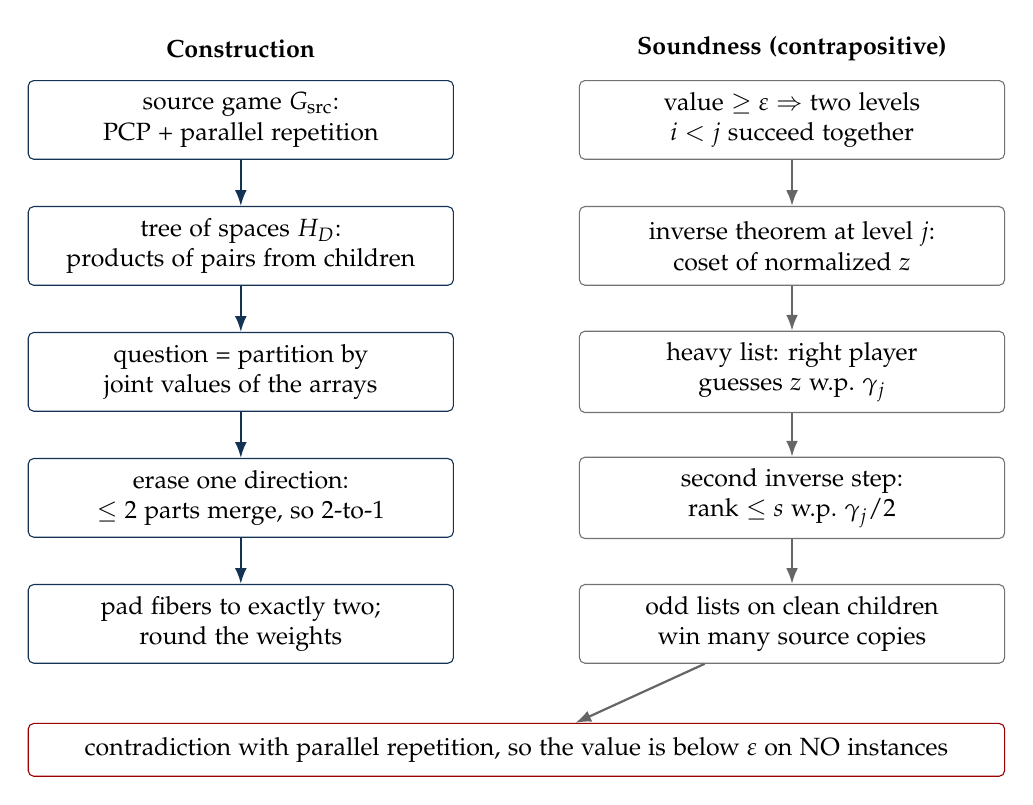
\begin{tikzpicture}[x=1cm,y=1cm,every node/.style={font=\small},
  box/.style={draw=linkblue!80!black,rounded corners=2pt,align=center,inner sep=4pt,minimum width=5.4cm,minimum height=10mm},
  sbox/.style={draw=black!55,rounded corners=2pt,align=center,inner sep=4pt,minimum width=5.4cm,minimum height=10mm},
  arr/.style={-{Latex[length=2mm]},thick,draw=linkblue!80!black},
  dsh/.style={-{Latex[length=2mm]},thick,draw=black!60}]
\node[font=\small\bfseries] at (0,0.9) {Construction};
\node[font=\small\bfseries] at (7,0.9) {Soundness (contrapositive)};
\node[box] (a) at (0,0) {source game $G_{\rm src}$:\\ PCP + parallel repetition};
\node[box] (b) at (0,-1.6) {tree of spaces $H_D$:\\ products of pairs from children};
\node[box] (c) at (0,-3.2) {question = partition by\\ joint values of the arrays};
\node[box] (d) at (0,-4.8) {erase one direction:\\ $\le2$ parts merge, so 2-to-1};
\node[box] (e) at (0,-6.4) {pad fibers to exactly two;\\ round the weights};
\draw[arr] (a)--(b); \draw[arr] (b)--(c); \draw[arr] (c)--(d); \draw[arr] (d)--(e);
\node[sbox] (f) at (7,0) {value $\ge\eps$ $\Rightarrow$ two levels\\ $i<j$ succeed together};
\node[sbox] (g) at (7,-1.6) {inverse theorem at level $j$:\\ coset of normalized $z$};
\node[sbox] (h) at (7,-3.2) {heavy list: right player\\ guesses $z$ w.p.\ $\gamma_j$};
\node[sbox] (i) at (7,-4.8) {second inverse step:\\ rank $\le s$ w.p.\ $\gamma_j/2$};
\node[sbox] (j) at (7,-6.4) {odd lists on clean children\\ win many source copies};
\draw[dsh] (f)--(g); \draw[dsh] (g)--(h); \draw[dsh] (h)--(i); \draw[dsh] (i)--(j);
\node[draw=red!60!black,rounded corners=2pt,align=center,inner sep=5pt,minimum width=12.4cm] (k) at (3.5,-8.0)
 {contradiction with parallel repetition, so the value is below $\eps$ on NO instances};
\draw[dsh] (j)--(k);
\end{tikzpicture}
\caption{Architecture of the proof.}
\label{fig:arch}
\end{figure}

\subsection{Status}

The manuscript is 53 pages. The repository lists a Lean formalization of the
main theorem: a Comparator statement \texttt{PerfectCompleteness.lean}
formalizing the reduction from binary 3SAT, with value exactly~$1$ on
satisfiable inputs and at most~$\delta$ otherwise. The check permits only
Lean's standard axioms, so no theorem enters the formal proof as an
assumption. The Lean development (about 580 files) proves its own versions of
the ingredients the paper cites, and its inverse theorem comes from the
release's Unique Games library rather than from the Khot--Minzer--Safra paper.
I have not run the check. On paper, the proof uses three external theorems as
black boxes: Dinur's PCP with perfect completeness \cite{Dinur}, the
Dinur--Steurer parallel repetition bound \cite{DS}, and the
Khot--Minzer--Safra Grassmann expansion theorem \cite{KMS18}.
\Cref{sec:reader} lists what to look at first.
Statement numbers such as ``Lemma~5.3'' refer to the compiled manuscript.

\section{The construction}\label{sec:construction}

Throughout, $\Fb$ is the two-element field and all vector spaces are over
$\Fb$.

\subsection{The source game}\label{sec:source}

Dinur's PCP with perfect completeness \cite{Dinur}, followed by routine local
encodings, maps a 3CNF formula to a 3CNF formula $\Psi$ with clauses on three
distinct variables. If the input is satisfiable, so is $\Psi$; if not, every
assignment violates a $\gamma_0$ fraction of clauses (Theorem~2.1). The
\emph{clause-versus-variable game} $G_\Psi$ asks the left player a clause $c$
and the right player one of its variables, chosen at random. The left answer
lies in $\Omega_c$, the seven satisfying assignments of $c$; the right answer
is a bit; and the constraint checks agreement. Its value is at most
$1-\gamma_0/3$ on NO instances. The \emph{source game} is the $t$-fold power
\[
 G_{\rm src}=G_\Psi^{\otimes t},
\]
whose value is at most $(1-\gamma_0^2/144)^t$ by Dinur--Steurer \cite{DS}
(Theorem~2.2). The power $t$ is fixed late in the parameter order. Answer sets
have sizes $7^t$ and $2^t$.

One small fact is used repeatedly. Each $\Omega_c$ projects onto all of
$\Fb$ in any single coordinate and onto all of $\Fb^2$ in any two
coordinates, since a clause excludes only one of eight triples.
\emph{Pair-surjectivity} makes the canonical form of a question below
well-defined.

\subsection{A tree of function spaces}\label{sec:tree}

Fix a depth $d$, branching numbers $n_1,\ldots,n_d$, row counts
$\ell_1,\ldots,\ell_d$ and product counts $R_1,\ldots,R_d$. Let $\cT$ be the
rooted tree with root at level $d$, leaves at level $0$, and $n_p$ children at
every level-$p$ node. A tuple $E$ of left source questions, one per leaf,
gives each leaf $C$ an answer domain $\Omega_C(E)$, a product of $t$ clause
domains. For a node $D$, $\Omega_D(E)$ is the product of the leaf domains below
it. Different leaves are \emph{always} separate coordinates, even when they
carry the same clause.

\begin{definition}[Definition~3.1]\label{def:spaces}
At a leaf $C$, $H_C$ is the space of \emph{all} functions $\Omega_C\to\Fb$.
For any node $C$ let $H_C^2=\Span\{gh:g,h\in H_C\}$ (pointwise products).
At an internal node,
\[
 H_D=\sum_{C\text{ child of }D}H_C^2\ \subseteq\ \Fb^{\Omega_D},
\]
where a function on a subtree is extended by ignoring the other coordinates.
\end{definition}

\begin{example}[What the spaces look like]
A leaf space is closed under products, so at level $1$ the space $H_D$
consists of sums of functions each depending on a single leaf. At level $2$,
products of two such functions from one level-1 child depend on at most two
leaves under that child. In general every element of $H_D$ at level $p$ is a
sum of products of at most $2^{p-1}$ single-leaf functions. Each product
follows a nested binary pattern: at every level only two pieces are
multiplied, each coming from a single child. So $H_D$ is \emph{contained in},
but generally smaller than, the span of all such products. Degree doubles at
each level, but every term stays inside a single child of $D$. That locality
is what the sampler and the clean-children argument exploit.
\end{example}

The basic properties (Lemma~3.2) are immediate: every space contains $1$,
$H_C\subseteq H_C^2$, and
\begin{equation}\label{eq:descendant}
 H_C^2\subseteq H_D\qquad\text{for every proper descendant $C$ of $D$}.
\end{equation}
Equation~\eqref{eq:descendant} is the structural heart of the construction.
\emph{A product of two functions displayed at a descendant is available at
every ancestor.}

\paragraph{Projected questions.} The analysis also uses \emph{mixed} tuples $O$
in which some leaf clause questions are replaced by their variable questions
along source edges. The coordinate projection
$\pi:\Omega_D(E)\to\Omega_D(O)$ is surjective. Pullback along it therefore
embeds $H_D(O)$ into $H_D(E)$, preserving pointwise products. We identify $H_D(O)$ with its image.

\subsection{Arrays, joint values, and questions as partitions}\label{sec:keys}

At each internal node $D$ at level $p$ the verifier chooses an \emph{array}
$M_D\in K_p\otimes H_D$, with $K_p=\Fb^{\ell_p}$. An array is a list of $\ell_p$
functions in $H_D$, called its \emph{rows}. On an assignment $x\in\Omega(E)$
to all leaves, the arrays give the joint value
\[
 \Psi_{E,\mathbf M}(x)=\bigl(M_D(x)\bigr)_{D\text{ internal}}
   \in\prod_D K_{\mathrm{level}(D)}.
\]
The honest prover wants to answer with $\Psi(x)$ for a satisfying assignment
$x$. The question is how to pose this so that the prover cannot exploit the
names of the functions, and so that left and right questions can be shared
across different representations. The manuscript's answer is to pose the
question as an \emph{unlabeled partition}.

\begin{definition}[Canonical key; Lemma~3.3]\label{def:key}
For a function $f$ on a product domain, discard every coordinate (leaf slot)
that $f$ ignores. Replace a clause slot by a single bit $u_j$ whenever $f$
depends on that slot only through one fixed position $j$, uniformly in all
other arguments. The resulting reduced domain carries typed coordinates:
full clause slots with their clause ID, and bit slots with their variable ID.
The \emph{key} of $f$ consists of a side tag (left or right), these typed
coordinates, and the \emph{unordered} partition $\mathcal P_f$ of the reduced
domain into the nonempty fibers of $f$. A legal answer is a part
$P\in\mathcal P_f$. Its \emph{restored output} $\out_f(P)$ is the common value
of $f$ on $P$.
\end{definition}

Pair-surjectivity makes the reduced position unique when it exists: a slot
that factors through two positions is constant, hence unused. The key depends
only on the equivalence relation $f(x)=f(x')$, not on names of output values.
Two consequences drive everything.
\begin{itemize}
\item \textbf{Sharing} (Lemma~3.4). If $f$ is defined on a projected domain
$\Omega(O)$, then $f$ and its pullback $f\circ\pi$ have \emph{literally the
same key}. A projected slot that $f$ uses becomes, for $f\circ\pi$, a clause
slot reducible to the projected position. So a question built on variable
questions is the same vertex as the corresponding question on clause
questions. This identification lets the analysis switch between $E$ and $O$
without the prover noticing.
\item \textbf{Joint legality.} Every legal answer is a part, so a single
assignment $x$ realizes \emph{all} of the restored block outputs at once. A
prover cannot give mutually inconsistent answers about different arrays.
\end{itemize}

The global quantifier in the reduction rule matters. The function
$f(x,b)=(1+b)x_1+bx_2$ on $\Omega_c\times\Fb$ reads one clause position for each
fixed $b$, but no single position for all $b$, so its clause slot is kept in
full.

\subsection{The one-bit test and perfect completeness}

For an internal node $D$ at level $p$ and a nonzero $a\in K_p$, let $Q_{D,a}$ be
the quotient $K_p\to K_p/\langle a\rangle$ at block $D$, and the identity
elsewhere. The \emph{edge} joins the left key of $f=\Psi_{E,\mathbf M}$ to the
right key of $g=Q_{D,a}\circ f$, with map
\[
 \pi_{f,D,a}(P)=\out_g^{-1}\bigl(Q_{D,a}\,\out_f(P)\bigr).
\]

\begin{lemma}[Lemma~3.5]\label{lem:two-fibers}
Each such map is a surjection with at most two preimages per right label. For
a fixed labeling, the edge accepts exactly when the restored outputs agree
through $Q_{D,a}$.
\end{lemma}

\begin{proof}
Restoration is a bijection between parts and attained values on each side,
and every attained $g$-value comes from an attained $f$-value. The kernel of
$Q_{D,a}$ on the whole output space is $\{0,(a\text{ at }D)\}$, so each fiber
of $Q_{D,a}$ has two elements, and its intersection with $\operatorname{im}f$
has at most two.
\end{proof}

\begin{proposition}[Perfect completeness; Proposition~3.6]\label{prop:completeness}
If the source instance is satisfiable, one labeling satisfies every edge.
\end{proposition}

\begin{proof}
Fix a satisfying assignment $\xi$ of the source variables. At any key, set
each retained clause coordinate to the triple given by $\xi$ and each
retained bit coordinate to its value under $\xi$. Label the key by the part
containing this point. The rule reads only the key, so it is consistent
across all edges that share a vertex. For an edge, both endpoints are labeled
by parts containing the reduction of the same point $x_\xi\in\Omega(E)$. The
restored outputs are therefore $f(x_\xi)$ and $g(x_\xi)=Q_{D,a}f(x_\xi)$, and
the edge accepts.
\end{proof}

The fibers have size \emph{at most} two. \Cref{sec:finish} pads them to
exactly two at a cost of $\delta/3$ in soundness.

\subsection{Exact identities forced by joint answers}\label{sec:identities}

Shifting an upper row by products of lower rows does not change the joint
partition at all. This is ``folding'' adapted to products.

\begin{lemma}[Joint folding; Lemma~3.7]\label{lem:folding}
Replace row $h$ of $M_D$ by $(M_D)_h+b_h$, where
\[
 b_h=c_h\cdot1+\sum_{C,u,v}\lambda_{h,C,u,v}\,(M_C)_u(M_C)_v
\]
for proper internal descendants $C$ of $D$. The new array family has
\emph{the same key}, and a fixed label's restored outputs change by
\[
 \widetilde y_C=y_C\ (C\neq D),\qquad
 (\widetilde y_D)_h=(y_D)_h+c_h+\sum\lambda_{h,C,u,v}(y_C)_u(y_C)_v.
\]
\end{lemma}

\begin{proof}
By \eqref{eq:descendant} the shift lies in $H_D$. On the output product, the
map that adds the displayed polynomial in the other blocks to block $D$ is an
involution, since its inputs are unchanged and the characteristic is two. The
new joint function is this bijection composed with the old one. The two
therefore have the same equality relation, the same reduced domain and the
same partition. Evaluating on any point of a part gives the formula.
\end{proof}

\begin{lemma}[Joint evaluation; Lemma~3.8]\label{lem:joint-eval}
Fix a legal response with restored outputs $y_C$ and a node $D$. On
\[
 B=\Span\bigl(\{1\}\cup\{(M_C)_u(M_C)_v: C\text{ a proper internal descendant of }D\}\bigr)
   \subseteq H_D
\]
there is a unique linear functional $b_y$ with $b_y(1)=1$ and
$b_y\bigl((M_C)_u(M_C)_v\bigr)=(y_C)_u(y_C)_v$. Every extension
$z\in H_D^*$ of $b_y$ has $z(1)=1$, and
\[
 \bigl(z((M_C)_u(M_C)_v)\bigr)_{u,v}=y_Cy_C^{\mathsf t},
 \qquad\text{a matrix of rank at most one.}
\]
\end{lemma}

\begin{proof}
One assignment $x$ realizes the whole response. Point evaluation at $x$,
restricted to $B$, has the required values and respects every linear relation
among the generators. The generators span $B$, so this fixes $b_y$. Extend
arbitrarily from a basis of $B$.
\end{proof}

\begin{idea}[Why this is the right invariant.]
Lemma~\ref{lem:joint-eval} is the algebraic certificate the soundness proof
looks for. An honest answer is evaluation at a point, and evaluation at a
point is multiplicative, so its ``product form'' $F(g,h)=z(gh)$ is a rank-one
matrix $yy^{\mathsf t}$ on every tested list of rows. A cheating prover is
forced to produce \emph{some} functional with this property on the rows it
was shown. The rest of the proof upgrades ``rank one on the tested rows'' to
``bounded rank everywhere'', which decodes to source answers.
\end{idea}

\subsection{The test distribution}\label{sec:sampler}

The arrays on the random path are not uniform. They come from a recursive
product sampler, which the manuscript calls its own redesign. Only the
underlying low-rank bucket viewpoint is credited to Golowich \cite{Golowich},
as mediated by Fei--Minzer--Wang \cite{FMW}. The sampler's structural purpose
is this. Every array above a node $D_p$ of the path is a
fixed polynomial expression in a bounded number of independent draws at $D_p$
(Lemma~4.1). That bound depends on the row and product counts but not on any
branching number.

\begin{enumerate}
\item Sample a left source question independently at each leaf, giving $E$.
\item Sample a uniformly random root-to-leaf path
$\mathsf P=(D_d,D_{d-1},\ldots,D_0)$.
\item The scalar sampler $\mathrm{Sample}(D_p)$, at a path node with path child
$C_*$, returns
\[
 \sum_{C\neq C_*}U_C\;+\;\sum_{h=1}^{R_p}G_hH_h,
 \qquad U_C\sim\mathrm{Unif}(H_C^2),\quad G_h,H_h\sim\mathrm{Sample}(C_*),
\]
with fresh randomness for every call. At a leaf it returns a uniform element
of $H_{D_0}$.
\item At a path node $D_p$ the array is a sum of \emph{buckets}
\[
 M_{D_p}=\sum_{v\in K_p\setminus\{0\}}v\otimes h_{p,v},
 \qquad h_{p,v}\sim\mathrm{Sample}(D_p)\text{ independently.}
\]
Arrays at nodes off the path are uniform.
\item Choose a level $p\in[d]$ uniformly and a direction $a_p\in K_p\setminus\{0\}$
uniformly. The edge joins the left key of $\Psi_{E,\mathbf M}$ to the right
key of $Q_{D_p,a_p}\Psi_{E,\mathbf M}$.
\end{enumerate}

Each ingredient has a job in the analysis:
\begin{itemize}
\item \textbf{Products of pairs} make the law of a sampled function have
\emph{small bias}, and the bound is independent of dimension
(\cref{lem:bias}). This feeds the Fourier heavy-list argument.
\item \textbf{Many children} hide which child is on the path. After a cut at
$D_p$ is ``stopped'', the observed data are close in total variation to
uniform (\cref{lem:hidden-child}).
\item \textbf{Buckets} realize a uniform rank-one step exactly once the cut
has been made uniform (\cref{sec:comparisons}). In that law, resampling the
bucket $h_a$ changes $M$ by $a\otimes h$ with $h$ uniform, which is the step
of the Grassmann/shortcode inverse theorem.
\item \textbf{Bounded stopped expressions} make the hiding estimates independent
of branching. They also let the clean-children argument zero out a
predetermined, bounded family of draws.
\end{itemize}

\begin{figure}[t]
\centering
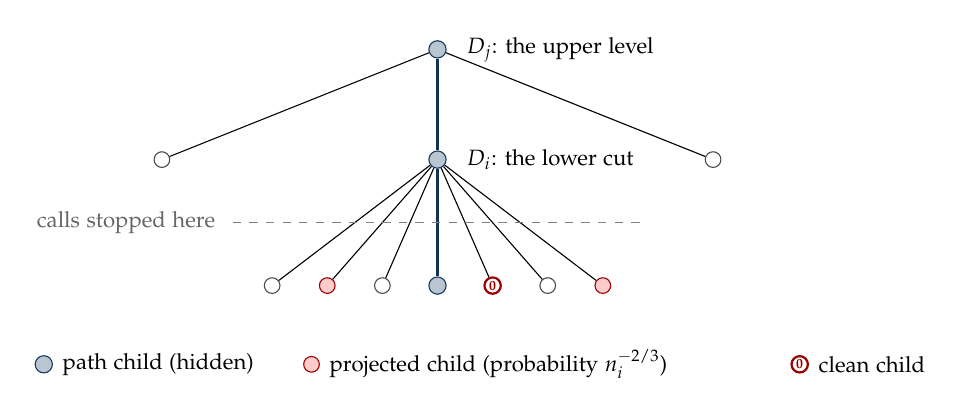
\begin{tikzpicture}[x=1cm,y=1cm,every node/.style={font=\footnotesize},
  nd/.style={circle,draw=black!70,inner sep=2pt,fill=white},
  pth/.style={circle,draw=linkblue!90!black,inner sep=2.2pt,fill=linkblue!30},
  prj/.style={circle,draw=red!60!black,inner sep=2pt,fill=red!20},
  cln/.style={circle,draw=red!60!black,thick,inner sep=0.6pt,fill=white,font=\tiny\bfseries,text=red!60!black}]
\node[pth] (r) at (0,0) {};
\node[anchor=west] at (0.25,0) {$D_j$: the upper level};
\node[nd] (a1) at (-3.5,-1.4) {}; \node[pth] (a2) at (0,-1.4) {}; \node[nd] (a3) at (3.5,-1.4) {};
\draw (r)--(a1); \draw[very thick,draw=linkblue!80!black] (r)--(a2); \draw (r)--(a3);
\node[anchor=west] at (0.25,-1.4) {$D_i$: the lower cut};
\foreach \k/\x/\s/\t in {1/-2.1/nd/{},2/-1.4/prj/{},3/-0.7/nd/{},4/0/pth/{},5/0.7/cln/0,6/1.4/nd/{},7/2.1/prj/{}}{
  \node[\s] (b\k) at (\x,-3.0) {\t}; \draw (a2)--(b\k);}
\draw[very thick,draw=linkblue!80!black] (a2)--(b4);
\draw[dashed,draw=black!50] (-2.6,-2.2)--(2.6,-2.2);
\node[anchor=east,text=black!60] at (-2.7,-2.2) {calls stopped here};
\node[pth,label={[font=\footnotesize]right:path child (hidden)}] at (-5.0,-4.0) {};
\node[prj,label={[font=\footnotesize]right:projected child (probability $n_i^{-2/3}$)}] at (-1.6,-4.0) {};
\node[cln,label={[font=\footnotesize]right:clean child}] at (4.6,-4.0) {0};
\end{tikzpicture}
\caption{The two levels in the soundness argument. Calls from above that
reach $D_i$ are ``stopped'' there. With many children, the path child is
statistically hidden. A sparse random set of children is projected, and a
clean child is a projected one all of whose contributions are zero.}
\label{fig:tree}
\end{figure}

\section{Two toolkits}\label{sec:tools}

The soundness proof uses two independent bodies of machinery. The first is
the matrix form of the Grassmann/shortcode inverse theorem. The second
consists of distributional comparisons for the sampler.

\subsection{The inverse theorem for matrix tables}\label{sec:inverse}

Let $K=\Fb^\ell$ and let $H$ be a finite space, so that a matrix
$M\in K\otimes H$ is a list of $\ell$ rows in $H$. The \emph{rank-one step}
takes a uniform $M$ to $M+a\otimes h$, with $a\in K\setminus\{0\}$ and
$h\in H$ uniform and independent. Both endpoints are uniform. A \emph{row and
column slice} is a nonempty affine set
\[
 \{M: AM=U,\ Mq_b=t_b\ (b\le c)\},
\]
which specifies some row combinations and some column values.

\begin{theorem}[Inverse theorem; Theorem~2.6]\label{thm:inverse}
For every $\eta>0$ there are $\alpha>0$ and integers $r,\ell_0$ such that for
all $\ell\ge\ell_0$, every finite space $H$, every finite set $\mathcal Y$
and every partial table $f:K\otimes H\to\mathcal Y\cup\{\bot\}$ the following
holds. If
\[
 \Pr_{M,a,h}\bigl[f(M)=f(M+a\otimes h)\neq\bot\bigr]\ \ge\ \eta,
\]
then some value $y\in\mathcal Y$ has density at least $\alpha$ on a slice
with at most $r$ row and $r$ column constraints. The constants do not depend
on $\dim H$ or $|\mathcal Y|$.
\end{theorem}

The proof has three short steps on top of the Khot--Minzer--Safra theorem: a
set of Grassmann vertices that retains a constant fraction of its edges (so
is far from pseudorandom) is dense in an interval of bounded co-order
\cite{KMS18} (Theorem~2.3).
\begin{enumerate}
\item \textbf{Chart} (Lemma~2.4, following \cite{BKS}). Send $M$ to its
graph $L_M=\{(x,M^{\mathsf t}x)\}\subseteq\Fb^\ell\oplus\Fb^m$. Then
$\dim(L_M\cap L_{M'})=\ell-\rank(M-M')$, so neighbors in the chart are
exactly rank-one changes. A vertex has $(2^\ell-1)(2^{m+1}-2)$ Grassmann
neighbors: choose one of the $2^\ell-1$ hyperplanes of $L_M$, then one of
the $2^{m+1}-2$ lines of the $(m+1)$-dimensional quotient that differ from the
image of $L_M$. Of these,
$(2^\ell-1)(2^m-1)$ stay in the chart, \emph{exactly half}. Retention
therefore drops by at most a factor of two. Containment of $A_0$ and
containment in $B_0$ translate into row and column equations.
\item \textbf{Dummy columns} (Lemma~2.5). The KMS theorem needs large ambient
dimension, but $H$ may be tiny, even zero. Pad with dummy columns. A slice in
the padded space projects to a slice in the original one, and \emph{every}
point has the same number of lifts, so densities are preserved exactly.
\item \textbf{Many values} (Theorem~2.6). With $\mu_y$ the mass of the
fiber $f^{-1}(y)$ and $\theta_y$ its retention, the defined-equality
probability equals $\sum_y\mu_y\theta_y$. Since $\sum_y\mu_y\le1$, some single
fiber has $\theta_y\ge\eta$. No factor $|\mathcal Y|$ is lost; this averaging
is also in \cite{BKS}. The chart is from \cite{BKS} as well. The
dummy-column elimination and the many-fibers lemma below are the
manuscript's own.
\end{enumerate}

The independence from $|\mathcal Y|$ is essential: the upper table's
responses record every lower block, so its range is enormous. The analysis
also needs a slice that a player can \emph{find} from random row advice.

\begin{lemma}[Many good row fibers; Lemma~2.7]\label{lem:many-fibers}
Let $\alpha,r$ be the constants of \cref{thm:inverse} at threshold $\eta/2$.
If a partial table has defined-equality probability at least $\eta$, then a
uniform
$A\in\Hom(K,\Fb^r)$ and an independent uniform $M$ satisfy: with probability
at least $(\eta/4)2^{-r\ell}$, the row fiber $\{M':AM'=AM\}$ contains a slice
(at most $r$ further column constraints) on which a single value has density
$\alpha$. The witness is a deterministic function of $(f,A,AM)$.
\end{lemma}

\begin{proof}[Proof idea]
Erase $f$ on the union $T$ of all good row fibers. If $T$ had measure below
$\eta/4$, the erased table would still have defined equality above $\eta/2$,
so the inverse theorem would produce a good fiber of the erased table. That
fiber lies in $T$, where the erased table is undefined, a contradiction.
Average over the $2^{r\ell}$ row maps.
\end{proof}

\subsection{Comparisons for the sampler}\label{sec:comparisons}

The analysis repeatedly replaces the true sampling law by simpler ones. Each
replacement is justified for a specified \emph{observation}, and the
bookkeeping of what may be observed is the subtle part.

\paragraph{Stopping at a cut (Lemma~4.1).} Fix the path down to a node $D_p$.
Each scalar call above $D_p$ is a sum of uniform functions from ordinary
children and $R_h$ products of two fresh calls to the path child. Stop every
call when it reaches $D_p$. Every ancestor array is then a fixed polynomial
expression in an \emph{exterior record} and at most
\[
 T_p=\sum_{k=p}^d(2^{\ell_k}-1)\prod_{h=p+1}^k 2R_h
\]
pending draws at $D_p$. Crucially, $T_p$ does not depend on any branching
number.

\paragraph{One hidden child (Lemma~4.2).} Each draw at $D_p$ and each array
below it decomposes into independent \emph{child blocks} $X_C$, one per child
$C$ of $D_p$. Under the true law, the block of the (unknown) path child $J$ has
some law $Q_C$, while every other block is uniform ($P_C$). Each block lives in
a space whose dimension depends only on lower parameters, so the density
$q_C=dQ_C/dP_C$ is at most a constant $L_p$.

\begin{lemma}\label{lem:hidden-child}
Forgetting the path below $D_p$, the true law of the blocks is within total
variation $L_p/(2\sqrt{n_p})$ of the uniform law.
\end{lemma}

\begin{proof}
The true density with respect to $P=\prod_C P_C$ is
$Z=\frac1{n_p}\sum_C q_C(X_C)$, an average of independent mean-one variables.
Then $\E_P(Z-1)^2=n_p^{-2}\sum_C\E(q_C-1)^2\le L_p^2/n_p$, and
$\TV\le\frac12\sqrt{\chi^2}$.
\end{proof}

The bound is lost if the observation reveals $J$, and much of the care in the
manuscript goes into never revealing it. In the uniform law the array at
$D_p$ is uniform, and resampling one bucket $h_a$ gives \emph{exactly} the
uniform rank-one step $M\mapsto M+a\otimes(h_a+h_a')$.

\paragraph{Sparse projection (Lemma~4.3).} At a lower cut $D_i$, mark each child
independently with probability $\beta_i=n_i^{-2/3}$. At every leaf of a marked
child, replace the clause question by a variable question, sampled
conditionally as in a source edge. Make all draws at the cut uniform in the
\emph{projected} spaces. Viewed through the pullback to the original domains,
the resulting \emph{modified} law is close to uniform:
\[
 1+\chi^2=\prod_C\bigl(1+\beta_i^2\chi^2(Q_C\Vert P_C)\bigr)
 \le(1+\beta_i^2L_i^2)^{n_i}\le\exp(L_i^2n_i^{-1/3}).
\]
This is a form of the Khot--Safra sub-code covering idea \cite{KS}.

\paragraph{Posterior of a selected child (Lemma~4.4).} Bayes' rule gives, for
every child and every observed lifted data,
\[
 \Pr(C\text{ marked}\mid\text{data})
 =\frac{\beta_iq_C}{1-\beta_i+\beta_iq_C}\le\frac{\beta_iL_i}{1-\beta_i}=:q_i.
\]
This holds even for a child chosen \emph{after} looking at the data. A useful
consequence: if two bilinear forms on $H_{D_i}(E)$ are determined by the
lifted data and differ, a witness pair lies in the square spaces of at most
two children. If neither child is marked, their restrictions to the projected
space also differ. So
\[
 \Pr\bigl(F_0\ne F_1,\ F_0|_{H'}=F_1|_{H'}\bigr)\le 2q_i.
\]

\paragraph{Small bias independent of dimension (Lemma~4.5).} Call a law on a
space \emph{quarter-balanced} if every nonzero linear functional takes each
value with probability at least $1/4$.

\begin{lemma}\label{lem:bias}
If $g,h$ are independent draws from quarter-balanced laws and $B$ is a nonzero
bilinear form, then $|\E(-1)^{B(g,h)}|\le7/8$. Consequently, if every
$R_p\ge R_{\min}$ (an absolute constant), every scalar law is
quarter-balanced, and every nonzero character has bias at most $(7/8)^{R_p}$
at level $p$.
\end{lemma}

\begin{proof}
The kernel of $g\mapsto B(g,\cdot)$ is a proper subspace, so some nonzero
functional vanishes on it, and quarter balance gives
$\Pr(B(g,\cdot)\neq0)\ge1/4$. Given such $g$, the bit $B(g,h)$ takes each value
with probability at least $1/4$. Each value of $B(g,h)$ therefore has
probability at least $1/16$, and the bias is at most $7/8$.

For the induction, let $f\ne0$ on $H_{D_p}$. If $f$ is nonzero on an ordinary
child's square space, the uniform summand makes $f(\cdot)$ an unbiased bit.
Otherwise $f$ is nonzero on the path child's square space, so $B(g,h)=f(gh)$
is a nonzero bilinear form there. Each of the $R_p$ independent products then
contributes a factor at most $7/8$.
\end{proof}

The bound uses only whether certain maps are nonzero, so no dimension enters.
This is why the Fourier argument of \cref{sec:upper} survives function spaces
whose dimension grows with the source alphabet.

\section{Soundness I: two levels and an upper decoder}\label{sec:upper}

Fix a labeling that, on a NO instance, accepts with probability at least
$\eps$. The goal of this and the next two sections is a contradiction.

\subsection{Two levels that succeed together}

Let $\mathrm{Acc}_p$ be acceptance of the test at level $p$, with all
directions sampled at once, and let $N=\sum_p\one_{\mathrm{Acc}_p}$. By
Jensen, $\E[N(N-1)]\ge(\E N)^2-\E N\ge d^2\eps^2-d\eps$. If $d\eps\ge4$,
averaging over the $d(d-1)$ ordered pairs gives levels $i<j$ with
\[
 \Pr(\mathrm{Acc}_i\cap\mathrm{Acc}_j)\ \ge\ \eps^2-\eps/d\ \ge\ \tfrac34\eps^2 .
\]
Pass to the \emph{modified} law at level $i$, in which children of $D_i$ are
sparsely projected and draws at $D_i$ are uniform. With branching large, this
costs at most $\eps^2/4$, leaving $\Pr_i(\mathrm{Acc}_i\cap\mathrm{Acc}_j)\ge
c:=\eps^2/2$.

Two levels are needed because each level supplies something the other lacks.
Success at the \emph{upper} level $j$ gives the inverse-theorem structure.
Success at the \emph{lower} level $i$ ties that structure to the lower rows,
on which joint legality certifies rank one, and to the projected children,
where the right player lives.

\subsection{The upper table}

Let $H=H_{D_j}(E)$ and $M=M_{D_j}$. The inverse theorem needs a table on
$K\otimes(\text{something})$ under the rank-one step. The difficulty is that
the response at $M$ depends on lower rows, and the analysis must not reveal
which level-$i$ node is on the path. The manuscript therefore lets
\[
 B=\Span\bigl(\{1\}\cup\{s_{C,t}s_{C,u}: C\text{ any level-$i$ descendant of
 }D_j\}\bigr)\subseteq H
\]
include the products of displayed rows at \emph{every} level-$i$ descendant, and
works on $H/B$. Choose a linear section $s:H/B\to H$. The table
$f_P(\bar M)$ queries the labeling with upper array $s(\bar M)$ and records the
whole response: the upper output $u$ and every lower output $y_C$.
\Cref{lem:folding} recovers the response at the true $M$, because
$M-s(\bar M)$ has rows in $B$. The upper output becomes $u+(M-s(\bar M))b_y$,
and the lower outputs are unchanged. Responses where level-$i$ success has
conditional probability below $c/2$ are marked undefined.

\begin{lemma}[Lemma~5.1]
Resampling the bucket of $M$ in the omitted direction $a$ produces two arrays
$M,M'=M+a\otimes h$. The partial table has defined equality at least $c^2/8$
on them, and at least $\theta=c^2/16$ under the uniform rank-one step on
$K\otimes(H/B)$.
\end{lemma}

\begin{proof}[Why]
The right question at level $j$ sees only $M$ modulo $\langle a\rangle$, so it
is the same for both draws. Successful left responses therefore agree with it,
and up to the folding correction, which also moves only along $a$, there are
at most two possible defined responses. Two independent draws coincide with
probability at least $(p_1+p_2)^2/2$, and Cauchy--Schwarz finishes. In the
uniform law at the upper cut, bucket resampling is exactly the rank-one step.
\end{proof}

\subsection{The coset of functionals}

Put $\eta=\theta/2=c^2/32$, so that with probability at least $\eta$ over the
lower data the table has defined equality at least $\eta$. Apply
\cref{lem:many-fibers} with random row advice $A\in\Hom(K,\Fb^r)$. With
probability at least $g=(\eta^2/4)2^{-r\ell}$ the advice is good. Its witness consists
of at most $r$ column functionals $q_a\in(H/B)^*$, values $v_a$, and a
response $t_*=(u,(y_C)_C)$ that occurs with density $\alpha$ on the slice.
Pull the $q_a$ back to $H$ and let $Z=\Span\{q_a\}\subseteq\Ann(B)$. The
response $t_*$ defines $b_y$ on $B$ as in \cref{lem:joint-eval}. Define
$z_0\in H^*$ to be $b_y$ on $B$ and $0$ on $s(H/B)$. At every match the
restored upper output is $Mz_0+u$, and \emph{every} $z$ in the coset $z_0+Z$
satisfies
\[
 z(1)=1,\qquad\bigl(z(s_{C,t}s_{C,u})\bigr)_{t,u}=y_Cy_C^{\mathsf t}
 \quad\text{for every level-$i$ descendant }C.
\]
So the left player has a whole coset of normalized functionals, each with
tested rank at most one at every lower node. Lemma~5.2 records the
quantitative form. Let $J$ be the event ``good advice and the column values
match''. Then
\[
 \Pr_i\bigl(J,\ R_j=Mz_0+u\bigr)-\rho\Pr_i(J)\ \ge\ b,
 \qquad \rho=\kappa\alpha/4,\quad b=\kappa\alpha q_0/4,
\]
where $R_j$ is the level-$j$ block restored from the right answer of the
level-$i$ test, and $q_0=g2^{-r\ell}$.
The difference form matters. Disintegrating it over the exposed data gives,
with probability at least $b$, a slice of positive mass on which the
conditional prediction probability is at least $\rho$. That is exactly the
hypothesis of the heavy-list lemma.

\subsection{What each player sees}

The proof now builds two \emph{local} decoders: a left one that sees only
left-player information, and a right one that sees only right-player
information. Split $M=M_{\rm known}+X$, where $X=\sum_{v\in\ker A\setminus0}
v\otimes h_v$ collects the buckets that the row advice cannot see.
\begin{itemize}
\item The \textbf{left input} $\mathcal L$ is $E$, the path through $D_i$, $A$,
all other arrays (including the full lower array $S=M_{D_i}$), and the known
buckets. It does \emph{not} include the omitted lower direction $a_i$.
\item The \textbf{right input} $\mathcal R$ is $O$, the path, $A$, $a_i$,
the other arrays on projected domains, the known buckets, and $S$ only
modulo $a_i$.
\item Neither player sees $X$. Its law $\mu_{\mathcal R}$ is computable from
the right input alone, and it is \emph{exactly} the conditional law given both
inputs, because hidden buckets use fresh, disjoint randomness. By
\cref{lem:bias}, every nonzero character of $X$ has bias at most
$\lambda=(7/8)^{R_j}$.
\end{itemize}
The right player can evaluate $G_{\mathcal R}(X)$, the restored upper response
of its own level-$i$ query when the hidden part equals $X$.

\subsection{A heavy list that works for every witness}

\begin{lemma}[One heavy list; Lemma~5.3]\label{lem:heavy}
Let $\mu$ be a law on $V=W\otimes H'$ in which every nonzero character has
bias at most $\lambda$, where $\operatorname{codim}W\le r$. Let
$G:V\to K$, let $h_0=2^{-r\ell}$ and $\tau=\rho h_0/4$, and suppose
$2^{-(\ell-r)}<\rho/8$ and $\lambda\le\min(h_0/2,\tau^2/2)$. For
$\sigma\in K^*$ let
\[
 \mathcal H_\sigma=\bigl\{\Phi\in V^*:|\E_\mu[(-1)^{\sigma(G(X))}\chi_\Phi(X)]|\ge\tau\bigr\}.
\]
Then $|\mathcal H_\sigma|\le2/\tau^2$. Moreover, if on an affine slice
$\mathcal C=\{X|_Q=t_Q\}$ with $\dim Q\le r$ one has
$\Pr_\mu(G(X)=Xz'+k_0\mid\mathcal C)\ge\rho$, then for some $\sigma$ with
$\sigma|_W\ne0$ the list $\mathcal H_\sigma$ meets
$(\sigma|_W)\otimes z'+W^*\otimes Q$.
\end{lemma}

\begin{proof}[Proof sketch]
The slice indicator is an average of $|W^*\otimes Q|$ characters, and small
bias gives $\mu(\mathcal C)\ge h_0/2$. Expanding the event
$G(X)=Xz'+k_0$ over $\sigma\in K^*$, at most a $\rho/8$ fraction of the
$\sigma$ annihilate $W$. Some other $\sigma$ therefore correlates with the
character $(\sigma|_W)\otimes z'$ on the slice. Removing the slice indicator
by its character expansion leaves an unconditional correlation of at least
$\tau$ with a character in the stated coset. For the size bound, sum $m$
sign-aligned heavy characters and apply Cauchy--Schwarz:
$m^2\tau^2\le m+m^2\lambda$, using only that products of distinct characters
have bias at most $\lambda$.
\end{proof}

The lists depend only on the right player's input, not on the left player's
witness. That is what makes the decoding local.

\begin{proposition}[Upper decoding; Proposition~5.4]\label{prop:upper}
There are randomized local strategies, a left one on $\mathcal L$ returning a
bilinear form $F_L$ on $H_i=H_{D_i}(E)$ and a right one on $\mathcal R$
returning $F_R$ on $H_i'=H_{D_i}(O)$, such that
\[
 \Pr\bigl(F_R=F_L|_{H_i'\times H_i'}\bigr)\ \ge\ \gamma_j
 :=b\,2^{-\ell_j}\frac{\tau^2}2\,2^{-r}>0 .
\]
Every left output has the form $F_L(x,y)=z(xy)$ with $z(1)=1$ and
$\rank\bigl(F_L(S_t,S_u)\bigr)_{t,u}\le1$. The constant $\gamma_j$ does not
depend on the lower row count $\ell_i$, on any branching number, or on the
source alphabet.
\end{proposition}

\paragraph{The two decoders.} The \emph{left} decoder samples $z$ uniformly
from the coset $z_0+Z$ and outputs $F_L(x,y)=z(xy)$. On bad advice it outputs
point evaluation at a fixed legal assignment. The \emph{right} decoder picks
$\sigma\in K^*$ at random and a random $\Phi$ from $\mathcal H_\sigma$. It
fixes $h_\sigma\in W$ with $\sigma(h_\sigma)=1$, sets $z_R=\Phi(h_\sigma)$,
and outputs $F_R(x,y)=z_R(xy)$. When the witness is favorable, some list
element lies in $(\sigma|_W)\otimes z'+W^*\otimes Q$. Contracting it with
$h_\sigma$ lands in $z'+Q$, the restriction of the coset to the projected
space, and the left's uniform choice hits it with probability
$2^{-\dim Q}\ge2^{-r}$.

\begin{idea}[Order of quantifiers.]
The constant $\gamma_j$ depends only on $\eps$, the inverse-theorem constants
and $\ell_j$. It does not depend on the lower row count $\ell_i$. This is what
lets the parameters be chosen top down: first $\ell_j$, then $\gamma_j$, then
a lower row count $\ell_i$ large enough for the rank test of
\cref{sec:lower}.
\end{idea}

\section{Soundness II: from tested rank to full rank}\label{sec:lower}

The left form $F_L(x,y)=z(xy)$ has rank at most one \emph{on the displayed
lower rows} $S_1,\ldots,S_{\ell_i}$. That alone says little, because the
left decoder chose $z$ after seeing those rows. A form can be rank one on the
rows it was built around and still have huge rank. This section shows that a
positive fraction of the agreement nevertheless comes from forms of bounded
\emph{full} rank. The manuscript notes that Fei, Minzer and Wang have a close
analogue of this step \cite{FMW}.

Call $F$ \emph{admissible} at $S$ if $F(x,y)=z(xy)$ with $z(1)=1$ and
$\rank\Gram_F(S)\le1$, where $\Gram_F(S)=(F(S_u,S_v))_{u,v}$.

\subsection{Resampling in the lower fiber}

Suppose that high-rank agreement, with $\rank F_L>s$, has probability $h$.
Fix both players' random tapes, which preserves this probability, and erase
every left output that is not admissible or has rank at most $s$. The
argument has three steps.
\begin{enumerate}
\item \textbf{Same right view, two left views.} The right player sees $S$ only
modulo $a_i$. Draw $S$ and $S'$ independently from the same fiber
$S\bmod a_i$. The right answer is the same for both, so both left forms
restrict to it with probability $\E p^2\ge(\E p)^2=h^2$. As an unfiltered
law, the pair is just $S'=S+a_i\otimes l$ with $S,l$ uniform.
\item \textbf{Restrictions equal $\Rightarrow$ forms equal.} Both full left
forms are functions of the lifted data. By the posterior bound
(\cref{sec:comparisons}), unequal forms with equal restrictions to the
projected space have probability at most $2q_i$.
\item \textbf{Transfer to uniform.} The remaining event, full defined equality
$f(S)=f(S+a_i\otimes l)$, is a function of lifted data. It therefore
transfers to the unrestricted uniform law at a total-variation cost
$\upsilon_i$.
\end{enumerate}
The result is a partial table $f$ on $K_i\otimes H_i$ under the uniform
rank-one step, with defined equality at least
$h^2-2q_i-\upsilon_i$ (Lemma~6.1). Every defined output is admissible at its
own argument and has rank greater than $s$.

\subsection{High-rank forms fail the rank test on slices}

Apply \cref{thm:inverse} to this table. It returns one \emph{fixed} form $F$
that is the output on an $\alpha'$-dense part of an affine row/column slice.
Every such occurrence has $\rank F>s$ and $\rank\Gram_F(S)\le1$. The next
lemma says this is impossible. It is elementary and pleasant.

\begin{lemma}[Lemma~6.2]\label{lem:rank-slice}
Let $F$ be a bilinear form on $H$, and let $\mathcal A\subseteq H^\ell$ be a
nonempty slice with at most $r'$ row constraints and at most $r'$ column
constraints. If $\ell\ge2m+r'$, then for uniform $S\in\mathcal A$
\[
 \Pr\bigl[\rank\Gram_F(S)\le1\bigr]\ \le\
 (2^m-1)\,2^{-(\rank F-2r')}+\bigl[1+(2^m-1)^2\bigr]2^{-m^2}.
\]
\end{lemma}

\begin{proof}
An invertible change of rows $Y=TS$ turns the row constraints into ``the first
$a\le r'$ rows are fixed''. It does not change the rank of the Gram matrix,
since $\Gram_F(Y)=T\Gram_F(S)T^{\mathsf t}$. The column constraints say each
free row lies in a translate of $N=\bigcap\ker q_v$, a subspace of
codimension $c\le r'$, and the free rows are independent. Restricting $F$ to
$N\times N$ loses at most $2c$ in rank, so $t:=\rank F|_N\ge\rank F-2r'$.

Take two disjoint groups of $m$ free rows, $x_1,\ldots,x_m$ and
$y_1,\ldots,y_m$. The functionals $\lambda_u=F(x_u,\cdot)|_N$ are
independent, each uniform on a translate of the $t$-dimensional image of
$F|_N$. A nonzero combination $\sum e_u\lambda_u$ is uniform on such a
translate, hence zero with probability at most $2^{-t}$. A union bound over
the $2^m-1$ combinations shows the $\lambda_u$ are linearly independent
except with probability $(2^m-1)2^{-t}$. When they are independent, each
column $(F(x_u,y_v))_u$ is uniform in $\Fb^m$. The $m\times m$ cross matrix
is then uniform, and exactly $1+(2^m-1)^2$ of the $2^{m^2}$ matrices have rank
at most one. A rank-$\le1$ Gram matrix has a rank-$\le1$ cross submatrix.
\end{proof}

Choose $m$ so that the second term is below $\alpha'/2$, then $s$ so that
$2^{m-(s-2r')}<\alpha'/2$, then $\ell_i\ge 2m+r'$ (and at least the inverse
theorem's $\ell_0'$). The fixed form $F$ then passes the rank test on less
than an $\alpha'$ fraction of the slice, contradicting its density.

\begin{proposition}[Low-rank agreement; Proposition~6.3]\label{prop:low-rank}
With these choices and $n_i$ large,
\[
 \Pr\bigl[F_L|_{H_i'}=F_R,\ F_L\text{ admissible},\ \rank F_L\le s\bigr]
 \ \ge\ \gamma_j/2 .
\]
The cutoff $s$ and the row count $\ell_i$ depend only on $\gamma_j$.
\end{proposition}

\begin{idea}[What was gained.]
Before this step the left form was certified only on the rows the verifier
displayed. Now, with probability $\gamma_j/2$, it is a normalized product form
of rank at most $s$ on the \emph{entire} space $H_i$, and it agrees after
projection with a form the right player computed on its own. A bounded rank
on all of $H_i$ is what lets the form be read at individual leaves.
\end{idea}

\section{Soundness III: odd lists, clean children, and repetition}\label{sec:clean}

It remains to turn bounded-rank agreement into a strategy for the source
game, and to show that it wins too often.

\subsection{Reading a form at a leaf}

For a finite set $\Lambda$, let $\cO_s(\Lambda)$ be the subsets of odd size at
most $s$. For a map $\pi:\Lambda\to\Gamma$, the \emph{parity pushforward} is
\[
 \pi_{\rm odd}(L)=\{b\in\Gamma:\ |L\cap\pi^{-1}(b)|\text{ is odd}\}.
\]
The \emph{odd-list game} $G_{{\rm odd},s}$ is the source game with answers
in $\cO_s$ and constraints $\pi_{\rm odd}$. The same pushforward describes how Fourier characters
restrict in low-degree long-code analysis (Dinur--Guruswami).

\begin{lemma}[Lemma~7.1]\label{lem:odd}
\begin{enumerate}
\item $\pi_{\rm odd}$ maps $\cO_s(\Lambda)$ into $\cO_s(\Gamma)$, and
$\val(G_{{\rm odd},s})\le s^2\val(G_{\rm src})$.
\item If $F(x,y)=z(xy)$ on $H_i$ with $z(1)=1$ and $\rank F\le s$, then at
every leaf $\lambda$ below $D_i$ the set $\{a: z(e_a)=1\}$ is in
$\cO_s(\Lambda_\lambda)$, where $e_a$ is the indicator that the answer at
$\lambda$ is $a$.
\item If the leaf is projected by $\pi_e$ and $F'=F|_{H_i'}$, the
corresponding set for $F'$ is the parity pushforward of the left set.
\end{enumerate}
\end{lemma}

\begin{proof}
(1) The sizes satisfy $|\pi_{\rm odd}(L)|\equiv|L|\equiv1\pmod 2$, and each
element of $\pi_{\rm odd}(L)$ has its own nonempty, disjoint preimage in $L$,
so $|\pi_{\rm odd}(L)|\le|L|$. For the value bound, let each player answer
with a uniformly random element of its list. On an accepted list edge, every
right element has an odd, hence positive, number of preimages in the left
list. So some pair accepts with probability at least $s^{-2}$.

(2) The indicators $e_a$ lie in the leaf space and satisfy $e_ae_b=0$ for
$a\ne b$, $e_a^2=e_a$, and $\sum_ae_a=1$. Hence $(F(e_a,e_b))$ is diagonal with
entries $d_a=z(e_a)$. Its rank, the number of $a$ with $d_a=1$, is at most
$s$, and $\sum_ad_a=z(1)=1$, so that number is odd.

(3) The pullback of the right indicator $e_b'$ is $\sum_{\pi_e(a)=b}e_a$, so
$F'(e'_b,e'_b)=\sum_{\pi_e(a)=b}d_a$.
\end{proof}

This is the clean replacement for the usual ``decode a long code to a short
list'' step. The orthogonal idempotents $e_a$ diagonalize every product form,
and normalization $z(1)=1$ forces the decoded list to be odd and hence
nonempty.

\subsection{Clean children}

To apply parallel repetition, the proof needs \emph{independent} source edges
together with \emph{local} rules that answer them. The trouble is that each
player's input involves sampled functions that depend on all leaves. The
manuscript's device, which it traces to the zero-advice idea of
Khot--Minzer--Safra \cite[Remark~3.2]{KMS17}, is to find children whose
contributions vanish.

Write every one of the $T_i^{\rm cl}$ draws at the cut $D_i$ (the rows of
$S$ together with all stopped calls) as a sum of independent child
contributions $U_{q,C}\in H_C(O)^2$. A child $C$ is \emph{clean} if it is
projected, all its contributions $U_{q,C}$ are zero, and every array in its
subtree is zero.

\begin{lemma}[Exact clean law; Lemma~7.2]\label{lem:clean-law}
Given the exterior data, the clean indicators are independent, each with
probability exactly $\beta_ip_{0,i}$, where
\[
 p_{0,i}=2^{-T_i^{\rm cl}\dim(H_C'^2)-\sum_{D\preceq C}\ell_{\mathrm{level}(D)}\dim H_D'}
\]
is the \emph{same for every child and every choice of source questions}.
Conditional on all public data, the source edges at the designated (first)
leaves of the clean children are independent, each with the source
distribution $\mu$.
\end{lemma}

\begin{proof}[Why the law is exact]
A fully projected subtree has answer domain $\Fb^t$ at every leaf, whatever
the variable IDs are. Its function spaces, and hence their dimensions, depend
only on the shape of the subtree. The probability that a fixed number of
independent uniform vectors all vanish is therefore the same for every
question tuple. The constant factor cancels when conditioning on cleanliness,
so the edge tuple in a clean child keeps its product law.
\end{proof}

\begin{idea}[Why exactness matters.]
If the probability of being clean depended, even slightly, on the source
questions, conditioning on cleanliness would bias those questions, and the
repetition theorem would no longer apply. A merely positive lower bound would
not do; the manuscript stresses this point. Two facts make the probability
exactly constant. First, asking each child's contributions to vanish
separately, rather than their sum, makes cleanliness an event about that
child's own latent summands. These events are independent across children,
and cancellations or shared constants cannot affect them. Second, a fully
projected subtree has function spaces that depend only on its shape, because
repeated variable IDs still occupy separate coordinates. The probability is
therefore a dimension count that is the same for every question tuple.
\end{idea}

\begin{lemma}[Local reconstruction; Lemma~7.3]
After the public data are fixed, each player can rebuild its exact decoder
input from its own questions at the designated clean leaves. The left player
recovers $E$ from its clause questions; the right player recovers $O$ from
its variable questions.
\end{lemma}

The reason is that every sampled function ignores the arguments in clean
children. Clean contributions are zero, nonclean contributions live
elsewhere, and the functions that ignore those arguments form an algebra.
Canonicalization then discards the clean slots. The left decoder is run
without $a_i$ and the right decoder with $S$ only modulo $a_i$, exactly as
specified. The right player's heavy lists are computed from the fixed
reference law $\mu_{\mathcal R}$, so no small-bias claim is needed after
conditioning on cleanliness.

\subsection{The repetition bound}

\begin{proposition}[Proposition~7.4]\label{prop:clean}
If $\val(G_{\rm src})<1/(2s^2)$, then the bounded-rank agreement event
$\mathcal L_{i,j,s}$ of \cref{prop:low-rank} satisfies
\[
 \Pr(\mathcal L_{i,j,s})\ \le\ \Bigl(1-\frac{\beta_ip_{0,i}}{64}\Bigr)^{n_i}
 \ \le\ \exp\Bigl(-\frac{p_{0,i}}{64}\,n_i^{1/3}\Bigr).
\]
\end{proposition}

\begin{proof}
By \cref{lem:odd}, $\val(G_{{\rm odd},s})<1/2$. Conditional on the public
data with $k$ clean children, the reconstructed decoders, followed by reading
diagonal supports at the designated leaves, form local strategies for
$G_{{\rm odd},s}^{\otimes k}$. Whenever $\mathcal L_{i,j,s}$ occurs, they win
every coordinate. Dinur--Steurer with gap $1/2$ bounds this by
$(1-\frac1{64})^k$. Averaging $(63/64)^{|\mathcal C|}$ over independent clean
indicators gives
$\prod_C(1-\beta_ip_{0,i}+\frac{63}{64}\beta_ip_{0,i})=(1-\beta_ip_{0,i}/64)^{n_i}$,
and $n_i\beta_i=n_i^{1/3}$.
\end{proof}

The constant $p_{0,i}$ depends on the source power $t$, the row and product
counts, and branching \emph{below} level $i$, but not on $n_i$. Taking
$n_i^{1/3}>\frac{64}{p_{0,i}}\log\frac{4}{\gamma_j}$ makes the bound smaller
than $\gamma_j/4$, contradicting \cref{prop:low-rank}.

\section{Assembly: parameters, exact fibers, and weights}\label{sec:finish}

\subsection{The order of choices}

Every estimate above is uniform in the quantities chosen after it. The order
is the following (Section~8 of the manuscript):
\begin{enumerate}
\item From $\delta$: put $\eps=\delta/3$, choose depth $d$ with $d\eps\ge4$, and
set $c=\eps^2/2$, $\kappa=c/2$, $\eta=c^2/32$. Take the inverse-theorem
constants $\alpha,r,\ell_0$ at threshold $\eta/2$.
\item \textbf{Row counts, top down.} At level $j$, choose $\ell_j$ large enough
for every lower rank test required by levels above $j$, and with
$2^{-(\ell_j-r)}<\rho/8$. This determines $\gamma_j$. Then choose the product
count $R_j$ with $(7/8)^{R_j}\le\lambda_j$, above an absolute minimum.
\item \textbf{Rank cutoff.} Let $s$ be the largest of the cutoffs from
\cref{sec:lower}.
\item \textbf{Source power.} Choose $t$ with $\val(G_{\rm src})<1/(2s^2)$. This
fixes the alphabets. It changes the dimension of every function space, but no
earlier constant depends on dimension: that is the point of the
dimension-free inverse theorem, heavy list and bias bound.
\item \textbf{Branching, bottom up.} Choose cubes $n_1,n_2,\ldots,n_d$ one at a
time, in ascending order of level. At level $p$, the likelihood bound $L_p$ and the clean
probability $p_{0,p}$ depend only on what was fixed earlier. Large $n_p$
therefore makes all of $L_p/\sqrt{n_p}$, the sparse-projection error, the
posterior $q_p$, and the clean bound $\exp(-p_{0,p}n_p^{1/3}/64)$ as small as
needed. Higher branching only adds exterior data, so it cannot spoil an
earlier choice.
\end{enumerate}

\begin{figure}[h]
\centering
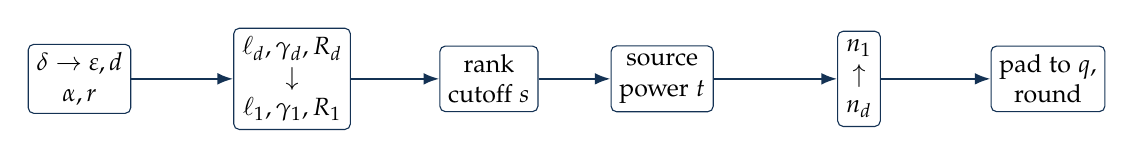
\begin{tikzpicture}[x=1cm,y=1cm,every node/.style={font=\small},
  bx/.style={draw=linkblue!80!black,rounded corners=2pt,align=center,inner sep=3pt,minimum height=8mm},
  ar/.style={-{Latex[length=2mm]},thick,draw=linkblue!80!black}]
\node[bx] (a) at (0,0) {$\delta\to\eps,d$\\$\alpha,r$};
\node[bx] (b) at (2.7,0) {$\ell_d,\gamma_d,R_d$\\$\downarrow$\\$\ell_1,\gamma_1,R_1$};
\node[bx] (c) at (5.2,0) {rank\\cutoff $s$};
\node[bx] (e) at (7.4,0) {source\\power $t$};
\node[bx] (f) at (9.9,0) {$n_1$\\$\uparrow$\\$n_d$};
\node[bx] (g) at (12.3,0) {pad to $q$,\\round};
\draw[ar] (a)--(b); \draw[ar] (b)--(c); \draw[ar] (c)--(e); \draw[ar] (e)--(f); \draw[ar] (f)--(g);
\end{tikzpicture}
\caption{The order in which the constants are fixed. Each estimate is
uniform in everything to its right.}
\label{fig:order}
\end{figure}

With these choices the preliminary game has perfect completeness, fibers of
size at most two, and value below $\eps$ on NO instances (Proposition~8.1).
Otherwise \cref{sec:upper} produces levels $i<j$ with agreement $\gamma_j$,
\cref{sec:lower} reduces it to bounded-rank agreement $\gamma_j/2$, and
\cref{sec:clean} bounds that by less than $\gamma_j/4$.

\subsection{Exactly two preimages}

The constraints so far are \emph{at most} 2-to-1 on legal answers. Embed all
legal answers in common alphabets $[2q]$ and $[q]$, where $q$ is large
compared with the constant bounds on legal answers and with $1/\delta$. For an
edge with legal map $\pi:L\to R$, every right label $b$ has residual capacity
$c_b=2-|\pi^{-1}(b)|$. The $N=2q-|L|$ illegal left labels are distributed into
these capacities in \emph{all} possible ways, each completion getting equal
weight. Every completion is exactly 2-to-1 and agrees with $\pi$ on legal
answers, so perfect completeness survives edge by edge. By symmetry, a fixed
illegal left label maps to a fixed right label with probability
$c_b/N\le2/N\le\delta/3$. Illegal answers can therefore add at most $\delta/3$
to the value.

\subsection{Removing weights}

All weights are rational with polynomial bit length. With $m$ weighted
entries, set $K=\lceil3m/\delta\rceil$ and replace weight $w_a$ by
$\lfloor Kw_a\rfloor$ copies, plus one copy for each of the first few entries
to bring the total to $K$. Only edges already in the support are used, so
completeness stays $1$. The total variation is at most $m/K\le\delta/3$. The
final soundness is $\eps+\delta/3+\delta/3=\delta$.

\section{Reader's guide}\label{sec:reader}

\paragraph{What is external.} Three theorems are used as black boxes:
\begin{itemize}
\item Dinur's PCP with perfect completeness \cite{Dinur};
\item the Dinur--Steurer bound $\val(G^{\otimes k})\le(1-g^2/16)^k$ for
projection games with value at most $1-g$ \cite{DS};
\item the Khot--Minzer--Safra theorem that pseudorandom sets in the Grassmann
graph expand near-perfectly \cite{KMS18}.
\end{itemize}
Everything else is proved in the manuscript, including the extensions of the
inverse theorem. The chart and the fiber averaging follow
Barak--Kothari--Steurer \cite{BKS}; the dummy-column and many-fibers lemmas
are new.

\paragraph{What is new relative to the 2-to-2 theorem.} A remark of mine,
not the manuscript's: the 2-to-2 reduction is built on linear equations over
$\Fb$, and satisfiable linear systems can be solved by Gaussian elimination.
That route therefore cannot have perfect completeness unless
$\mathsf P=\mathsf{NP}$, and repetition is unavailable for 2-to-1 games. The
manuscript instead starts from a satisfiable CSP and uses a test that an
honest prover passes
\emph{exactly}: questions are unlabeled partitions given by joint evaluation of
a tree of polynomial arrays, and one output direction is erased. Soundness
then rests on four mechanisms:
\begin{enumerate}
\item exact algebraic identities forced by joint legality;
\item a hidden-path sampler whose statistics are uniform in all dimensions;
\item a rank-promotion step, from tested rank one to bounded full rank;
\item an exactly balanced ``clean child'' event that recreates independent
source edges.
\end{enumerate}
The manuscript credits Golowich \cite{Golowich} and Fei--Minzer--Wang
\cite{FMW} for the bucket viewpoint and for an analogue of the rank step.

\paragraph{Where to look first.} The proof is long but modular, and its
information bookkeeping is unusually explicit. A referee should concentrate on
four places:
\begin{itemize}
\item \textbf{The information sets.} Section~5.3 of the manuscript defines
exactly what each decoder sees. The left decoder never receives the omitted
lower direction, and the right decoder receives the lower array only modulo
that direction. These restrictions are used again in the reconstruction of
Lemma~7.3, and the two descriptions must match.
\item \textbf{The comparison chain.} Each total-variation step (original
$\to$ modified at the lower cut $\to$ uniform at the upper cut) is valid only
for observations that do not reveal the hidden path or the projection marks.
The ``common observations'' paragraph in Section~4.3 states what may be
observed. Check that every event to which a comparison is applied is of that
kind.
\item \textbf{Disintegrations.} The proof is careful not to condition on
success before applying the posterior bound or the bias bound. Lemma~5.2 and
Proposition~5.4 disintegrate an unconditional inequality instead. This is the
point most likely to hide a slip.
\item \textbf{Exactness of the clean law.} Lemma~7.2 needs the cleanliness
probability to be literally independent of the source questions, which holds
because projected subtrees have identical function spaces. Check that the
padded call family really is fixed before the row advice selects visible
buckets.
\end{itemize}

\paragraph{Formal verification.} The result comes with a Lean
formalization: the Comparator challenge \texttt{PerfectCompleteness.lean},
whose solution is a development of about 580 Lean files, plus shared
libraries, in the repository's
\texttt{lean/} directory. The challenge permits only Lean's standard axioms
(\texttt{propext}, \texttt{Quot.sound}, \texttt{Classical.choice}), so none
of the external theorems is assumed. The formal route need not follow the
paper's citations: for example, its matrix inverse theorem is imported from
the release's Unique Games development. If the check passes, the remaining
question is whether the formal statement matches Theorem~1.1. I have not run
the check.


\begin{thebibliography}{99}\small
\bibitem{OAI} OpenAI. \emph{Perfect completeness for 2-to-1 games.} Manuscript, September 23, 2026. \url{https://github.com/openai/math}.
\bibitem{AOTW} P.~Austrin, R.~O'Donnell, L.-Y.~Tan, J.~Wright. New NP-hardness results for 3-coloring and 2-to-1 Label Cover. \emph{ACM Trans.\ Comput.\ Theory}, 2014.
\bibitem{BKS} B.~Barak, P.~Kothari, D.~Steurer. Small-set expansion in shortcode graph and the 2-to-2 conjecture. ITCS 2019 (ECCC TR18-077).
\bibitem{BKM} M.~Braverman, S.~Khot, D.~Minzer. On rich 2-to-1 games. ITCS 2021.
\bibitem{DMR} I.~Dinur, E.~Mossel, O.~Regev. Conditional hardness for approximate coloring. \emph{SIAM J.\ Comput.}\ 39(3), 2009.
\bibitem{Dinur} I.~Dinur. The PCP theorem by gap amplification. \emph{J.\ ACM} 54(3), 2007.
\bibitem{DKKMS} I.~Dinur, S.~Khot, G.~Kindler, D.~Minzer, M.~Safra. Towards a proof of the 2-to-1 games conjecture? STOC 2018; On non-optimally expanding sets in Grassmann graphs, STOC 2018.
\bibitem{DS} I.~Dinur, D.~Steurer. Analytical approach to parallel repetition. STOC 2014.
\bibitem{FMW} Y.~Fei, D.~Minzer, S.~Wang. On the hardness of 4-to-1 games with perfect completeness. ECCC TR26-179, September 2026.
\bibitem{Golowich} L.~Golowich. From Grassmannian to simplicial high-dimensional expanders. ECCC TR23-065, 2023.
\bibitem{GS} V.~Guruswami, A.~Sinop. Improved inapproximability results for maximum $k$-colorable subgraph. \emph{Theory of Computing} 9, 2013.
\bibitem{GSan} V.~Guruswami, S.~Sandeep. $d$-to-1 hardness of coloring 3-colorable graphs with $O(1)$ colors. ICALP 2020.
\bibitem{Hastad} J.~H{\aa}stad. On the NP-hardness of Max-Not-2. \emph{SIAM J.\ Comput.}\ 43(1), 2014.
\bibitem{Khot} S.~Khot. On the power of unique 2-prover 1-round games. STOC 2002.
\bibitem{KMS17} S.~Khot, D.~Minzer, M.~Safra. On independent sets, 2-to-2 games, and Grassmann graphs. STOC 2017.
\bibitem{KMS18} S.~Khot, D.~Minzer, M.~Safra. Pseudorandom sets in Grassmann graph have near-perfect expansion. FOCS 2018; \emph{Annals of Math.}, 2023.
\bibitem{KS} S.~Khot, M.~Safra. A two-prover one-round game with strong soundness. \emph{Theory of Computing} 9, 2013.
\bibitem{OW} R.~O'Donnell, Y.~Wu. Conditional hardness for satisfiable 3-CSPs. STOC 2009.
\bibitem{Raz} R.~Raz. A parallel repetition theorem. \emph{SIAM J.\ Comput.}\ 27(3), 1998.
\end{thebibliography}
\end{document}
